%************************************************
\chapter{Charge to Mass ratioe/m}
%************************************************
\begin{flushright}
January 8 and 15, 2012
\end{flushright}
\section{Aim}
	To determine the charge to mass ratio (e/m) of an electron by the helical method (long solenoid).
\section{Apparatus}
	e/m by Helical Method apparatus (we used the one by SIBA india), connecting wires

\section{Cathode Anode}
	Cathodes are defined to be where a reduction takes place (chemically). Thus in accordance with the <TODO: ADD IMAGE REFERENCE>, the anode is where the conventional current starts from and moves towards the cathode. For an electron, it starts from the cathode and moves towards the anode.
\section{Theory}
	Our objective here, as described earlier, is to determine the charge to mass ratio. For this, we shall describe here, an apparatus, without developing a motivation for doing the same.
	\par
	First, consider a vacuum tube; in one edge, say the starting edge (there's a screen at the other edge), we place a cathode and a perforated anode and apply a constant potential difference between them (the polarity is implied from the definition of cathode), such that the electrons move away from the starting edge. Now we can evaluate the speed of the electrons that pass through the anode by invoking the work energy theorem as follows:
	\begin{equation}
		\frac 1 2 mv^2 = eV
	\end{equation}
	where the symbols have their usual meaning, viz. $m$ is mass of electron, $v$ is speed of electron at the instant described, $V$ is the potential applied across the anode and cathode, and $e$ is the charge of one electron. Refer to the diagram for direction conventions assumed. If we try to turn on the apparatus at this stage, we should just see a spot, we assume to be the centre of the screen (this may not necessarily happen experimentally, but can be adjusted; however for simplicity, we will discuss that later)
	\par
	Now the next step is introducing a differential velocity component (do not confuse this with infinitesimal) along the $X$ direction. This is done by applying an alternating electric field as shown in the figure. When the electrons reach the plane A, they would have a certain distribution of velocity components along the $X$ direction. It is important to realize here that the distribution of electrons along the $X$ axis will be fairly small, because the velocities are not large enough to cause enough spatial deviation, in the small time corresponding to the length of the accelerating plates. This condition can be achieved by making the speed of the electrons sufficiently large with respect to the length of the alternating electric field plates. Yet, when observed on the screen, a line would be obtained (it's length would depend on the strength of the alternating electric field) as the electrons get displaced along (or against) the $X$ axis, as they're displaced by $L'$ along the $Z$ axis, because of the initial velocity.
	\par
	With that said, it is now that we introduce a uniform magnetic field B along the $Z$ axis. We are certainly introducing certain errors by doing so, as the magnetic field in the experiment is present everywhere in the tube, when it's turned on. However, to simplify, we account for it's effect after the electrons have passed the plane $A$.

\section{Observations and Calculations}
	\begin{table}
		\myfloatalign
		\begin{tabularx}{\textwidth}{Xlll}
			\hline
			\tableheadline{Order of Dark Ring $m$} 	&	\tableheadline{Left (cm)} & \tableheadline{Right (cm)}\\
			\hline
				6	&	5.800	&	6.260\\
				9	&	5.755	&	6.304\\
				12	&	5.720	&	6.350\\
				13	&	5.704	&	6.360\\
				14	&	5.700	&	6.370\\
				15	&	5.670	&	6.382\\
				16	&	5.665	&	6.400\\
				19	&	5.650	&	6.420\\
				23	&	5.605	&	6.459\\
				25	&	5.600	&	6.467\\
			\hline
		\end{tabularx}
		\caption{Diameter of Newton's Ring}
		\label{1_Diameter}
	\end{table}

	% \begin{figure}[bth]
	% 	\begin{center}
	% 		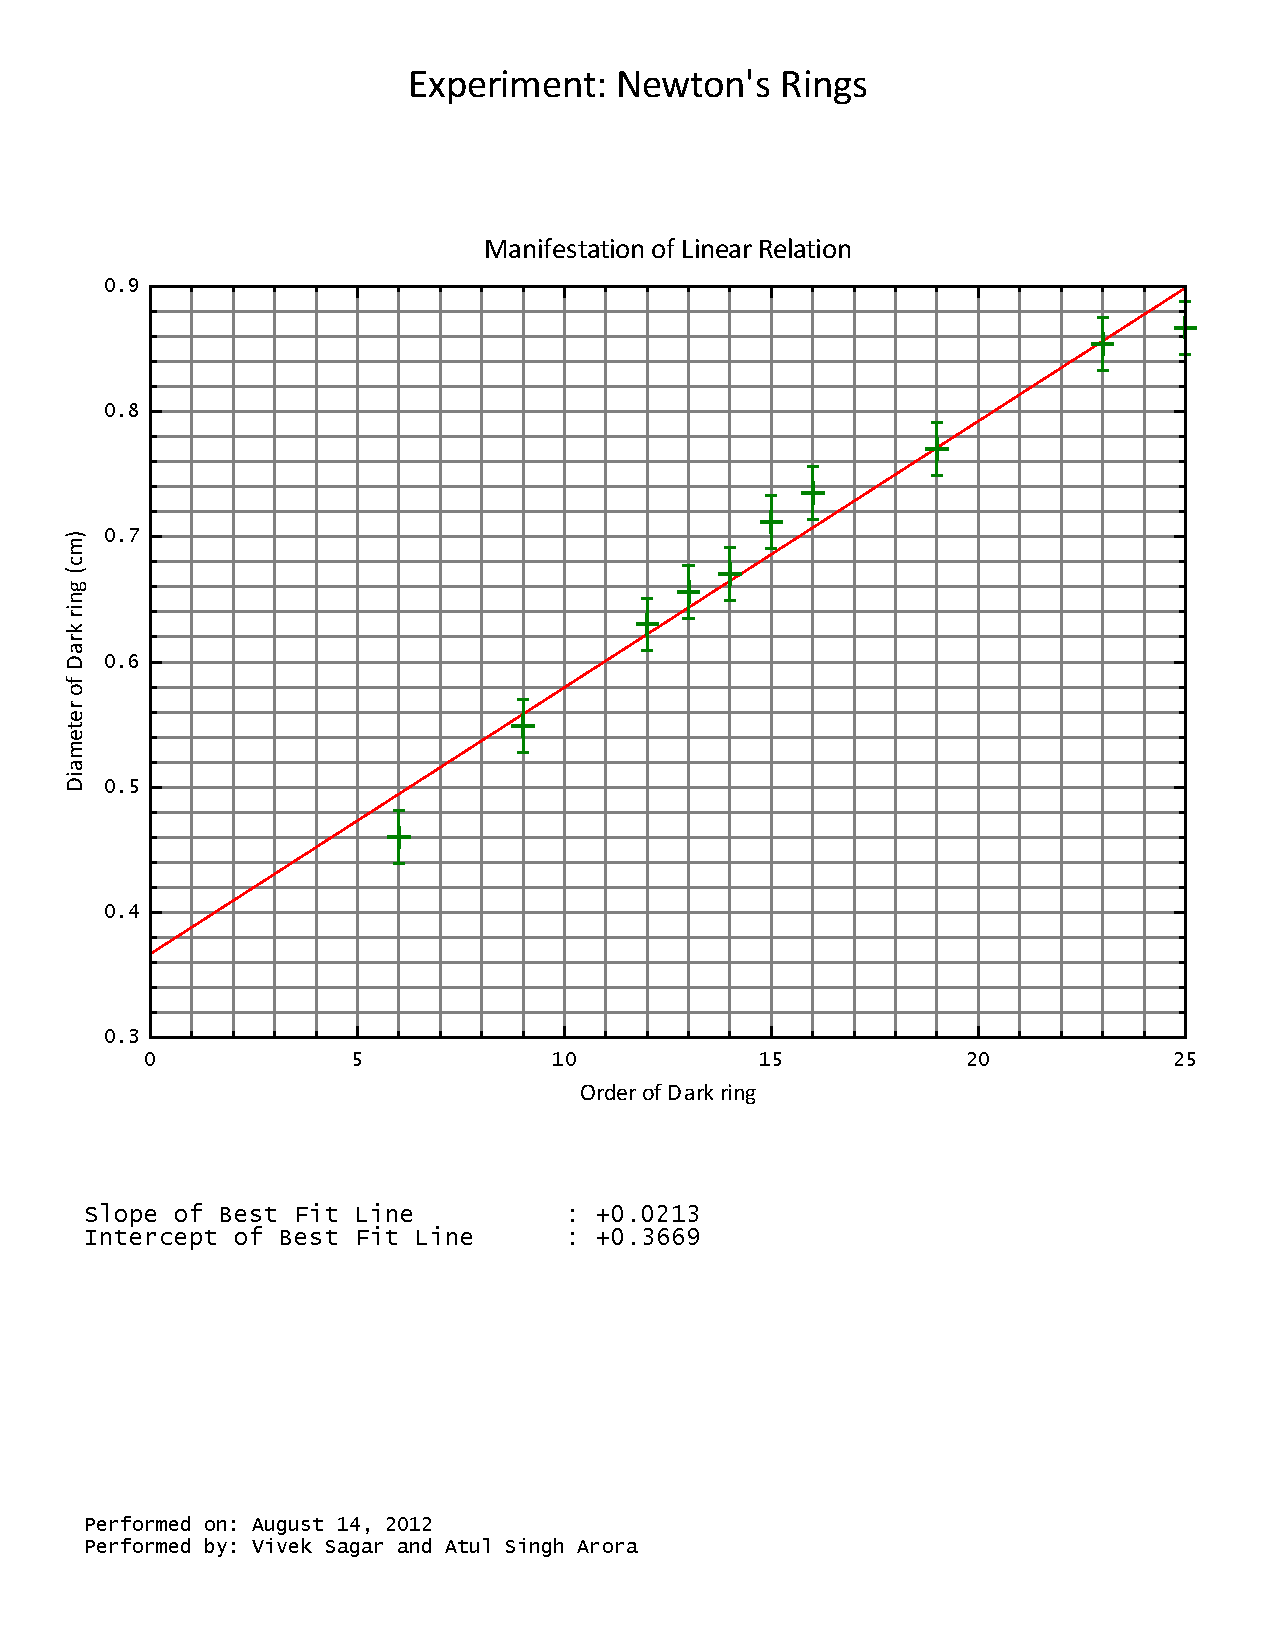
\includegraphics[width=1.3\linewidth]{gfx/1_linear.pdf}
	% 	\end{center}
	% \caption[Diameter Squared vs Order of Ring]{Least Square Fit of Diameter Squared vs Order of Ring}
	% \label{1_graph}
	% \end{figure}


\section{Result}
	The expected wavelength of sodium vapour lamp is $589.5$ nm. \\
	Experimentally, the wavelength, $\lambda$ was found to be \\
	$598.16\pm 3.25\%$ nm (standard deviation of the slope).\\
	Accuracy error is $1.5\%$, within the precision.
